\begin{figure}
  \centering
  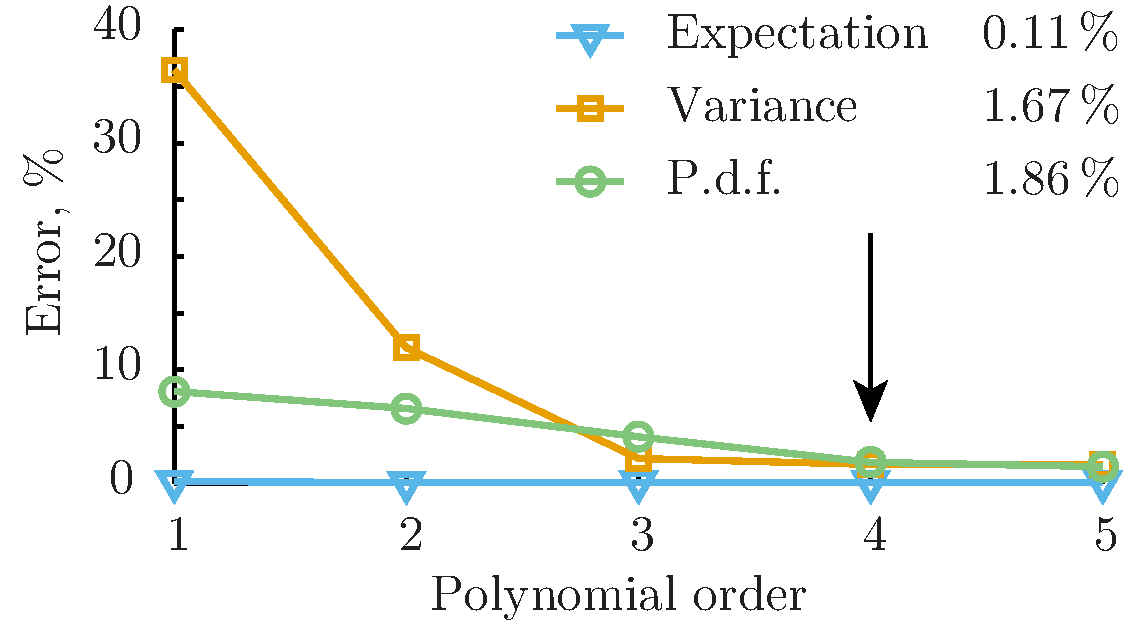
\includegraphics[width=1.0\columnwidth]{include/assets/accuracy.pdf}
  \caption{Errors of expectation, variance, and \pdf}
  \flabel{accuracy}
  \vspace{-1.6em}
\end{figure}

In this section, we report the results of the proposed framework for different configurations of the illustrative example in \sref{illustrative-example}.
All the experiments are conducted on a GNU/Linux machine with Intel Core i7 2.66~GHz and 8~GB of RAM.

Now we shall elaborate on the default configuration of our experimental setup, which, in the following subsections, will be adjusted according to the purpose of each particular experiment.
We consider a 45-nanometer technological process.
The effective channel length is assumed to deviate by 5\% from the nominal value of 45~nm where the global and local variations are equally weighted \cite{juan2011, juan2012}.
Correlation matrices are computed according to \eref{correlation-function} where the length-scale parameters $\ell_\SE$ and $\ell_\OU$ are set to half the size of the square die.
In the model order reduction technique (see \sref{ie-uncertain-parameters}), the threshold parameter is set to 0.99 preserving 99\% of the variance of the data.
Dynamic power profiles involved in the experiments are based on simulations of randomly generated, \via\ TGFF (v3.5) \cite{dick1998}, applications defined as directed acyclic task graphs.
The floorplans of the platforms are constructed in such a way that the processing elements form regular grids.\footnote{The task graphs of the applications, floorplans of the platforms, configuration of HotSpot, which was used to construct thermal RC circuits for our experiments, are available online at \cite{sources}.}
Time steps of power and temperature traces are set to 1 ms (see \sref{problem-formulation}).
To assess the performance of our polynomial chaos (PC) expansions, we employ a Monte Carlo (MC) sampling technique.
For each sample, \ie, for each outcome of the uncertain parameters, the MC approach solves the initial problem in \eref{fourier-system} numerically using the fourth- and fifth-order Runge-Kutta formulae \cite{press2007} available in MATLAB \cite{matlab}.

\subsection{Approximation Accuracy} \slabel{er-accuracy}
\begin{figure}
  \centering
  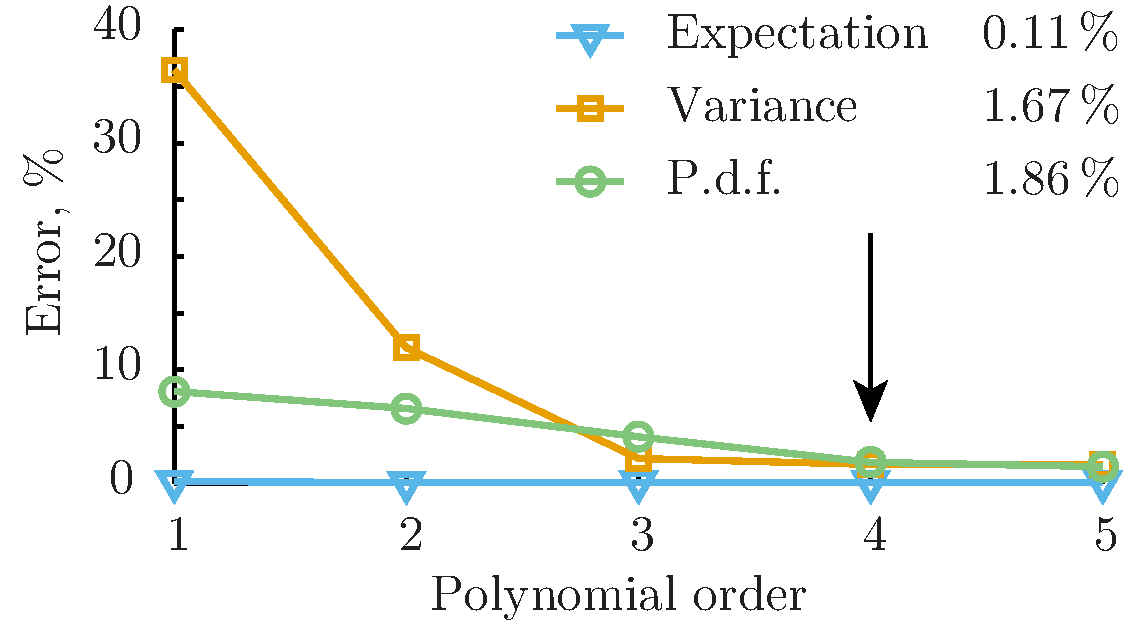
\includegraphics[width=1.0\columnwidth]{include/assets/accuracy.pdf}
  \caption{Errors of expectation, variance, and \pdf}
  \flabel{accuracy}
  \vspace{-1.6em}
\end{figure}


\subsection{Computational Speed} \slabel{er-speed}
\begin{table}[b]
  \vspace{-16pt}
  \centering
  \caption{Scaling with the number of processing elements $\cores$.}
  \begin{tabular*}{0.85\linewidth}{p{20pt}crrr}
    \toprule
    $\cores$ & $\vars$ & PC, seconds & MC, hours & Speedup, times \\
    \midrule
    $ 2$ & $2$ & $ 0.32$ & $31.24$ & $3.55 \times 10^5$ \\
    $ 4$ & $3$ & $ 0.45$ & $30.88$ & $2.46 \times 10^5$ \\
    $ 8$ & $4$ & $ 1.26$ & $31.44$ & $9.01 \times 10^4$ \\
    $16$ & $5$ & $ 6.55$ & $38.34$ & $2.11 \times 10^4$ \\
    $32$ & $6$ & $40.29$ & $41.58$ & $3.72 \times 10^3$ \\
    \bottomrule
  \end{tabular*}
  \tlabel{scaling-cores}
  \vspace{5pt}
  \caption{Scaling with the number of steps $\steps$.}
  \begin{tabular*}{0.85\linewidth}{p{42pt}rrr}
    \toprule
    $\steps$ & PC, seconds & MC, hours & Speedup, times \\
    \midrule
    $   10$ & $ 0.04$ & $   0.88$ & $8.19 \times 10^4$ \\
    $ 10^2$ & $ 0.06$ & $   3.12$ & $1.99 \times 10^5$ \\
    $ 10^3$ & $ 0.43$ & $  31.35$ & $2.65 \times 10^5$ \\
    $ 10^4$ & $ 4.35$ & $ 318.00$ & $2.63 \times 10^5$ \\
    $ 10^5$ & $42.23$ & $3110.29$ & $2.65 \times 10^5$ \\
    \bottomrule
  \end{tabular*}
  \tlabel{scaling-steps}
\end{table}

